\section{Eulerkredse og -veje}

En bestemt type af kredse gennemgår alle kanter i en graf og kaldes Eulerkredse. 

\begin{defn}\label{euler_def}
	En Eulerkreds er en simpel kreds i grafen $G$ som indeholder hver kant i $G$.
	En Eulervej er en simpel vej i grafen $G$, som indeholder hver kant i $G$.  
\end{defn}

\begin{exmp}
	Et eksemepel på en Eulerkreds og en Eulervej kan ses i Figur \ref{?} og \ref{?}: 
\end{exmp}

\begin{figure}[h]
\centering
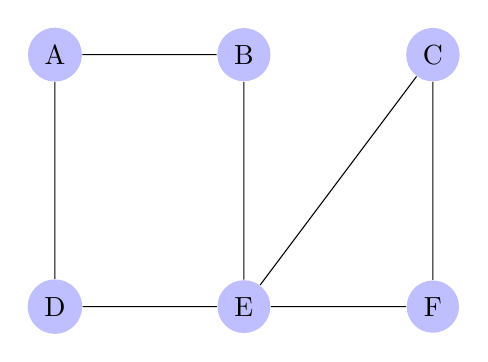
\begin{tikzpicture}
[scale=.8,auto=left,every node/.style={circle,fill=blue!25}]
  \node (n6) at (3,2) {D};
  \node (n4) at (3,6) {A};
  \node (n5) at (6,2) {E};
  \node (n1) at (6,6) {B};
  \node (n2) at (9,2) {F};
  \node (n3) at (9,6) {C};
  \foreach \from/\to in {n6/n4,n5/n1,n2/n5,n2/n3,n1/n4,n6/n5,n5/n3}
    \draw (\from) -- (\to);
\end{tikzpicture}
\caption{Euler kreds} 
\label{euler_kreds}
\end{figure}

\begin{figure}[h]
\centering
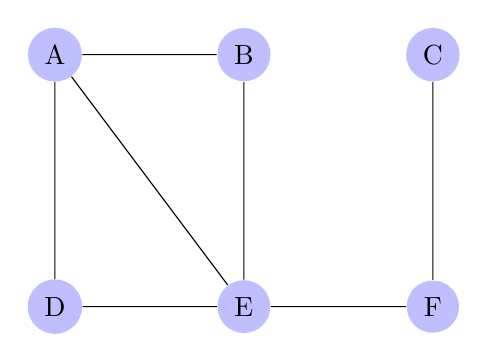
\begin{tikzpicture}
[scale=.8,auto=left,every node/.style={circle,fill=blue!25}]
  \node (n6) at (3,2) {D};
  \node (n4) at (3,6) {A};
  \node (n5) at (6,2) {E};
  \node (n1) at (6,6) {B};
  \node (n2) at (9,2) {F};
  \node (n3) at (9,6) {C};
  \foreach \from/\to in {n6/n4,n5/n1,n2/n5,n2/n3,n1/n4,n6/n5,n4/n5}
    \draw (\from) -- (\to);
\end{tikzpicture}
\caption{Euler vej} 
\label{euler_vej}
\end{figure}

Et eksempel på en Eulerkreds i Figur \ref{euler_kreds} kan være: $A,B,E,C,F,E,D,A$, og
et eksempel på en Eulervej i Figur \ref{euler_vej} kan være: $A,B,E,D,A,E,F,C$.

Der eksiserer ikke en Eulerkreds i alle grafer.

\begin{thm}\label{Eulerkreds_multigraf}
	En sammenhængende multigraf med mindst to knuder, har en Eulerkreds hvis og kun hvis, hver knude er af lige grad.
\end{thm}

\begin{proof} 
	Først bevises det at hvis en graf har en Eulerkreds, så er graden af alle knuderne i grafen lige. 

	En kreds begynder i en knude $a$ og fortsætter langs en kant, som er incident med $a$, til en ny knude $b$. 
	Denne kant kaldes $\lbrace a,b \rbrace$, og kanten bidrager med 1 til $\deg(a)$. 
	Hver gang kredsen passerer gennem en knude, tilføjes 2 til graden af denne knude. 
	Til sidst ender kredsen tilbage i $a$, og bidrager igen med 1 til $\deg(a)$.
	Hele graden af hver knude opnåes, da alle kanter skal passeres.  
	Derfor må $\deg(a)$ være lige og graden af hver knude må også være lige.  
	
	Nu bevises at hvis alle knuder er af lige grad, vil der eksistere en Eulerkreds i grafen.

	For at finde en Eulerkreds i en sammenhægende multigraf  $G$, som opfylder at graden af hver knude er lige, tages først udgangspunkt i en tilfældig underkreds i $G$.
	Denne underkreds starter i en knude $a$, hvorfra en simpel vej dannes ved at bevæge sig rundt i grafen. 
	Dette forsættes indtil en knude nås, hvorfra det ikke er muligt at komme videre, fordi alle incidente kanter allerede er en del af den simple vej, som nu er blevet til en kreds. 
	Herefter indførers $H$, som er lig med $G$, frataget kanterne i den tilfældige underkreds.
	Alle knuder i grafen vil stadig være af lige grad.
	Så dannes en ny underkreds i $H$, som starter i et endepunkt i den tidligere underkreds.
	Fordi grafen er sammenhængende vides det at den nye underkreds kan forbindes med en tidligere underkreds. 
	Kanter i den nye underkreds fjernes fra $H$. 
	Samtidig sættes de to underkredse sammen til én kreds.
	Denne procedure forsættes, indtil der ikke er flere kanter i $H$.
	Da må der være dannet en Eulerkreds. 
\end{proof} 
 
Proceduren kan ses i Algoritme \ref{algoritme_euler}.
Der findes også andre algoritmer, som kan finde Eulerkredse i en graf, men disse bliver ikke nævnt i dette projekt.
  
\begin{algorithm}
	\caption{Eulerkredse}
	\label{algoritme_euler}
	\textbf{procedure} Euler(G: sammenhængende multigraf med knuder af lige grad)\\
	$kreds:=$ en kreds i G der begynder i en vilkårlig knude med kanter, der danner en kreds.\\
	$H:= G$ med kanterne fra $kreds$ fjernet\\
	\textbf{så længe} $H$ har kanter\\
	$\-$ $\-$ $\-$ $\-$ $\-$ $\-$
	$underkreds:=$ en kreds i $H$, der begynder i en knude $v$ i $H$, som også er et endepunkt af en kant i $kreds$ \\ 
	$\-$ $\-$ $\-$ $\-$ $\-$ $\-$
	$H:=$ $H$ uden kanterne af $underkreds$ samt alle isolerede knuder fjernet \\
	$\-$ $\-$ $\-$ $\-$ $\-$ $\-$
	$kreds:=$ $kreds$ med $underkreds$ indsat \\ 
	\textbf{retuner} $kreds$ ($kreds$ er en Eulerkreds)
\end{algorithm}

\begin{thm}
Kompleksiteten af algoritmen for at finde en eulerkreds, er af lineær orden.
\end{thm}

\begin{proof}
For at finde algoritmens kompleksitet, opskrives en funktion, der beskriver antallet af sammenligner algoritmen laver for hver knude, $e$.
Der tages udgangspunkt i det værst mulige tilfælde. 
Hver gang algoritmen er ved en knude, vil den undersøge, om den kan vælge en kant, hvor den ikke allerede har været. 
Dette kræver en sammenligning per kant.
Finder algoritmen ved sammenligning, at den ikke kan vælge en kant, som den ikke har valgt før, vil den fjerne den underkreds der er dannet. 
Dette gør, at algoritmen må tage udgangspunkt i en ny knude, som er incident med en af kanterne i den fjernede underkreds.
I den nye knude vil algoritmen lave en ny sammenligning, for at finde ud af, om den kan vælge en kant, hvor den ikke har været før.
Dette vil betyde, at det værst mulige tilfælde vil være i en multigraf, hvor der hele tiden vil blive dannet underkredse bestående af to kanter. 
Hver gang algoritmen danner en ny underkreds, vil det kræve en ekstra sammenligning, og fordi dette sker hver anden gang i værste tilfælde, vil den endelige forskrift blive $f(e)=e+ \frac{e}{2}$.
Nu kan $O(g(e))$ findes:
\begin{align*}
f(e) = e+ \frac{e}{2} \\
\frac{e}{2} \leq 2e \\
f(e) \leq O(e).
\end{align*}
Derfor kan funktionen siges at være $O(e)$, med vidnerne $C=2$ og $k=1$.
Så findes $\Omega (g(e))$:
\begin{align*}
f(e) = e + \frac{e}{2} \\
\frac{e}{2} \geq e \\
f(e) \geq \Omega (e).
\end{align*}
Funktionen kan altså siges at være $\Omega (e)$, med vidnerne $C=1$ og $k=1$.
Da funtionen både er $O(e)$ og $\Omega (e)$ kan den også siges at være $\Theta (e)$.
\\\\
Hvis der ikke findes en Eulerkreds i en graf, kan der godt eksistere en Eulervej. 
\end{proof}

\begin{thm} \label{Eulervej_multigraf}
	En sammenhængende multigraf graf $G$ har en Eulervej, men ikke en Eulerkreds, hvis og kun hvis den har præcist to knuder af ulige grad.  
\end{thm} 

\begin{proof}
	Først bevises det at hvis der eksistere en Eulervej i en graf, vil netop to knuder være af ulige grad. 

	Antag at en sammenhængende multigraf, $G$, har en Eulervej fra $a$ til $b$, men ikke en Eulerkreds. 
	Den første kant som passeres på vejen bidrager med 1 til $\deg(a)$. 
	Hver gang vejen passerer knuden $a$ vil 2 tilføjes til $\deg(a)$. 
	Den sidste kant på vejen bidrager 1 til graden af endeknuden for vejen, $\deg(b)$. 
	Ligesom for $a$, kan vejen krydse $b$. 
	Hver gang dette måtte ske tilføjes 2 til graden af $b$. 
	Resultatet bliver, at $a$ og $b$ altid vil være af ulige grad. 
	Alle andre knuder på vejen vil være af lige grad, fordi 2 tilføjes til graden af en knude, hver gang en knude passeres.  
	
	Nu bevises det at vis der indgår netop to knuder af ulige graf i grafen, vil der eksistere en Eulerkreds.

	Antag at $a$ og $b$ er de eneste knuder af ulige grad. 
	Hvis en kant $\lbrace a,b \rbrace$ tilføjes til $G$, vil alle knuder i grafen være af lige grad. 
	Så gælder Sætning \ref{Eulerkreds_multigraf}, og der vil være en Eulerkreds i $G$. 
	Fjernes kanten $\lbrace a,b \rbrace$ igen vil der være en Eulervej. 
\end{proof}

\section{Hamiltonkredse og -veje}
En anden type kreds er en Hamiltonkreds. 
En Hamiltonkreds er en kreds som går gennem hver knude i grafen én gang. På samme måde kan der også eksistere en Hamiltonvej, som er en vej der går gennem hver knude i en graf én gang. 

\begin{defn} \label{hamiltion_defn}
	En Hamiltonvej er en simpel vej i en graf $G$, som går gennem hver knude én gang.
	En simpel kreds i en graf $G$, som går gennem hver knude én gang kaldes en Hamiltonkreds.
\end{defn}

\begin{exmp}
	Eksempler på en Hamiltonkreds og en Hamiltonvej kan ses i Figur \ref{?} og \ref{?}.
	
	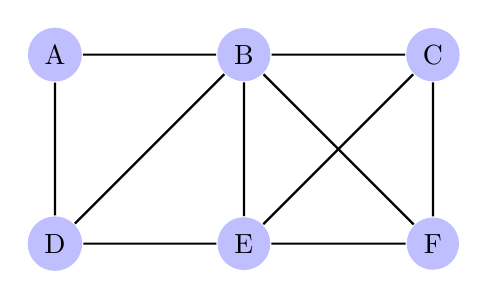
\begin{tikzpicture}
[thick,scale=.8,auto=left,every node/.style={circle,fill=blue!25}]
  \node (n6) at (3,2) {D};
  \node (n4) at (3,5) {A};
  \node (n5) at (6,2) {E};
  \node (n1) at (6,5) {B};
  \node (n2) at (9,2) {F};
  \node (n3) at (9,5) {C};
  \foreach \from/\to in {n6/n4,n4/n1,n6/n1,n6/n5,n1/n3,n1/n2,n1/n5,n5/n2,n5/n3,n3/n2}
    \draw (\from) -- (\to);
\end{tikzpicture}

	
	Et eksempel på en Hamiltonkreds i grafen er: $A,B,F,C,E,D,A$, og
	et eksempel på en Hamiltonvej er: $A,D,B,C,F,E$.
\end{exmp}

Der kendes ikke en simpel måde til at bestemme om der findes en Hamiltonkreds i en graf, ligesom der gør for en Eulerkreds. 
Der findes dog flere sætningerne der kan give en ide om eksistensen af en Hamiltonkreds. Med udgangspunkt i \citep{wilson_graph} og \citep{orebevis} bevises følgende to sætninger.

\begin{thm} \label{ores_thm}
	\textbf{Ores Sætning:} 
	Lad $G$ være er en simpel graf med $n$ knuder, og $n\geq3$, hvor er $\deg(u)+\deg(v)\geq n$ for hvert par af knuder, $u$ og $v$, der ikke er naboer i $G$. 
	Da har $G$ en Hamiltonkreds. 
\end{thm}

\begin{proof}
	Lad $G=(V,E)$ være en graf med $n$ knuder, som opfylder sætningens betingelser. For modstrid antages det, at denne graf \textit{ikke} indeholder en Hamiltonkreds.

	Til denne graf kan der tilføjes kanter uden at overtræde sætningens betingelser. Antag nu, at grafen $G$ mangler netop én kant, for at indeholde en Hamiltonkreds. 
	Da må $G$ indeholde Hamiltonvejen 
	$$v_1, v_2,...,v_n,$$
	som går gennem alle grafens knuder. 
	Men idet $G$ ikke indeholder en Hamiltonkreds, må $v_1$ og $v_n$ da \textit{ikke} være naboer.
	Derfor opfylder de, at
	\begin{align} \label{eq:sum_deg}
		\textrm{deg}(v_1)+\textrm{deg}(v_n)\geq n.
	\end{align}

	Der må være en knude $v_i$ der er nabo til $v_1$, som opfylder, at $v_{i-1}$ er nabo til $v_n$.
	Da kan de følgende to mængder opstilles:
	\begin{align*}
		A &= \lbrace i: 2 \leq i \leq n-1, \; v_1 \; \textrm{er nabo til} \; v_i \rbrace \\
		B &= \lbrace i: 3 \leq i \leq n, \; v_n \; \textrm{er nabo til} \; v_{i-1} \rbrace,
	\end{align*}
	hvor $A$ er mængden af indekser på knuder, $v_1$ er nabo til, og $B$ er mængden af indekser plus 1, på knuder, $v_n$ er nabo til. 

	Om disse gælder, at
	\begin{align*}
		|A| &= \deg(v_1) \\
		|B| &= \deg(v_n),
	\end{align*}
	hvorfor $A,B \subseteq \lbrace 2,...,n \rbrace$, som indeholder $n-1$ elementer.
	Fra Ligning \eqref{eq:sum_deg} må $\deg(v_1) + \deg(v_n) \geq n$.
	Skuffeprincippet giver så, at $A$ og $B$ deler mindst ét element, og der må da findes et $v_i$ og et $v_{i-1}$ som er forbundet til henholdsvis $v_1$ og $v_n$.

	\begin{figure}[h!]
		\centering
		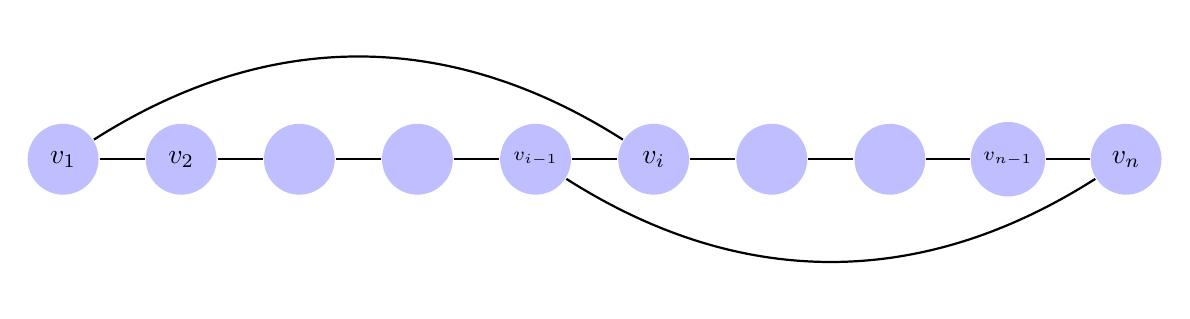
\begin{tikzpicture}                                         
[thick,auto,node distance=1.5cm,every node/.style={circle,minimum size=0.9cm,fill=blue!25}]
  \node (n1) {$v_1$};  
  \node (n2) [right of=n1] {$v_2$};
  \node (n3) [right of=n2] {};  
  \node (n4) [right of=n3] {};       
  \node (n5) [right of=n4] {\scriptsize $v_{i-1}$};
  \node (n6) [right of=n5] {$v_i$};
  \node (n7) [right of=n6] {}; 
  \node (n8) [right of=n7] {};         
  \node (n9) [right of=n8] {\scriptsize $v_{n-1}$};
  \node (n10) [right of=n9] {$v_n$};                                                
  \foreach \from/\to in {n1/n2,n2/n3,n3/n4,n4/n5,n5/n6,n6/n7,n7/n8,n8/n9,n9/n10}
    \draw (\from) -- (\to);
  \path                            
    (n1) edge [bend left=32.5] (n6)  
    (n10) edge [bend left=32.5] (n5);
\end{tikzpicture}

		\caption{En illustration der viser Hamiltonkredsen i $G$.} \label{ore_bevis}
	\end{figure}
	
	En Hamiltonkreds kan nu dannes af følgen $v_1, v_2,...v_{i-1},v_n,...,v_i,v_1$,
	som skitseres i Figur \ref{ore_bevis}. Dette er i modstrid med vores antagelse om, at der ikke eksisterer en Hamiltonkreds i en graf med de givne betingelser.	
\end{proof}

En anden sætning der kan bruges til at undersøge om der eksiserer en Hamiltonkreds i en graf er Diracs Sætning 

\begin{thm} \label{diracs_thm}
	\textbf{Diracs Sætning:} 
	Lad $G$ være en simpel graf med $n$ knuder, og $n\geq3$, så graden af hver knude i $G$ er mindst $\frac{n}{2}$, har $G$ en Hamiltonkreds.  
\end{thm}

\begin{proof}
	Lad $G=(V,E)$ være en graf med 3 eller flere knuder. Udvælg fra grafen, $G$, to knuder, $u$ og $v$, der ikke er naboer. Det følger da direkte af Ores Sætning, at
	\begin{align*}
	\textrm{deg}(u) + \textrm{deg}(v) \geq \frac{n}{2} + \frac{n}{2} = n,
	\end{align*}
	hvorfor grafen må have en Hamiltonkreds.
\end{proof}

Derudover gælder det også, at der ikke kan eksistere en hamiltonkreds i en graf med en knude, der har graden 1. 
Disse to sætninger beskriver, hvornår der med sikkerhed eksisterer en Hamiltonkreds, men en Hamiltonkreds kan godt eksistere uden at opfylde sætningerne. 

\begin{exmp}
	I Figur \ref{pentagon} ses en graf der indeholder en hamiltonlkreds.
	Grafen overholder ikke betingelserne i Ores' Sætning, da summen af to knuders grader aldrig kan give et resultat større end $4$, hvilket er mindre end $n$.
	Grafen overholder heller ikke betingelserne i Diracs Sætning, fordi $n=5$, mens graden af hver kant i grafen er $2$, hvilket er mindre end $n/2$.
	
	\begin{figure}[h]
	\centering
		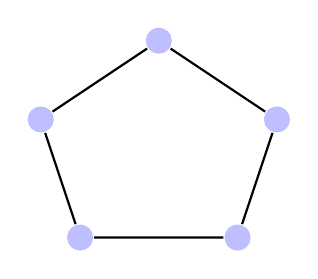
\begin{tikzpicture}[thick, every node/.style={shape=circle,fill=blue!25}]
	\path (0,0) node (p0) {}
	(-1.5,-1) node (p1) {}
	(-1,-2.5) node (p2) {}
	(1,-2.5) node (p3) {} 
	(1.5,-1) node (p4) {};
	\draw (p0) -- (p1)
	(p0) -- (p1)
	(p0) -- (p4)
	(p1) -- (p2)
	(p2) -- (p3) 
	(p3) -- (p4);    
\end{tikzpicture}                             

	\caption{Hamiltonkreds i en graf med 5 knuder}
	\label{pentagon}
	\end{figure}
\end{exmp}
%Et kendt probelm hedder...
%Der er blevet formuleret et problem, som kaldes Hamiltonvej Problemet eller Hamiltonkreds problemet. 
%Dette problem går ud på, at det ønskes at finde ud af om der eksisterer en hamiltonkreds eller -vej i en given graf. 

Problemet Hamiltonian Path Problem er et kendt, svært problem inden for grafteori. 
Dette problem går netop ud på at finde ud af, om der eksisterer en hamiltonvej eller -kreds i en given graf.

\begin{thm} \label{path_problem}
	Hamiltonian Path Problem er NP-fuldstændigt. \citep{computers}
\end{thm}

Der vil blive gjort brug af denne sætning i løbet af projektet, men denne vil ikke blive bevist. 
Der henvises til \citep{computers} for beviset.
